\section{Methodology}

\subsection{Pre-Processing}

To clean the data, it was first necessary to load the data into a pandas data frame. Sometimes the presence of erroneous data in pandas can accidentally give a data-frame column the wrong data-type. In the case of this data, one would expect columns 1 to 11 to be a float64 data type and int64 for the 12th quality column. Luckily pandas interpreted the data correctly so there was no need for correction. 

Next up, it was necessary to make sure there was no missing data in our dataset and that all data was numeric. The scope of this pre-processing phase was to find and eradicate any NAN or Null values. Luckily again none were identified.

Finally, it was necessary to look at a summary of our data frame using df.describe(). This gives a summary of the entire data frame with the count, min, max, std, and mean for all features. Here I was looking for any logical anomalies in the data. For example, a quality value greater than 10 or less than zero would be indicated here. Once again there were no anomalies that could be found in the dataset. 

\subsection{Correlation}

A heat map was used to get a quick visual representation of the entire dataset and its correlated features.

\begin{figure}[H]
\centering
        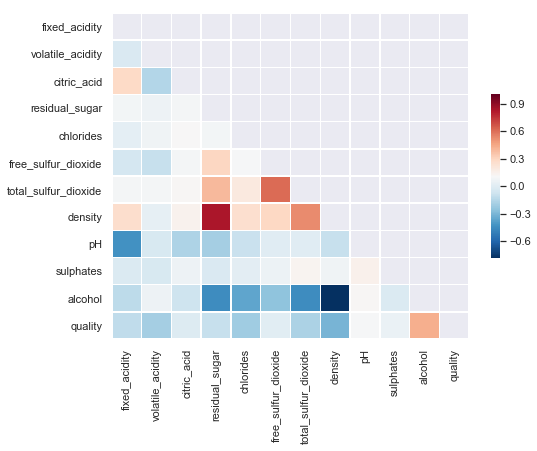
\includegraphics[totalheight=8cm]{images/correlation.png}
    \caption{Heatmap depicting correlated features.}
    \label{fig:heatmap}
\end{figure}

In figure \ref{fig:heatmap} it is clear that density and residual sugar are both highly correlated features. This high correlation could cause problems with the classification model, So I decided to remove residual sugar from the dataset to make processing faster and to decrease harmful bias in the model.

\subsection{Outliers}

Boxplots were used to try and identify outliers. Figure \ref{fig:boxplot-all} shows a box plot for all features in the dataset

\begin{figure}[H]
\centering
        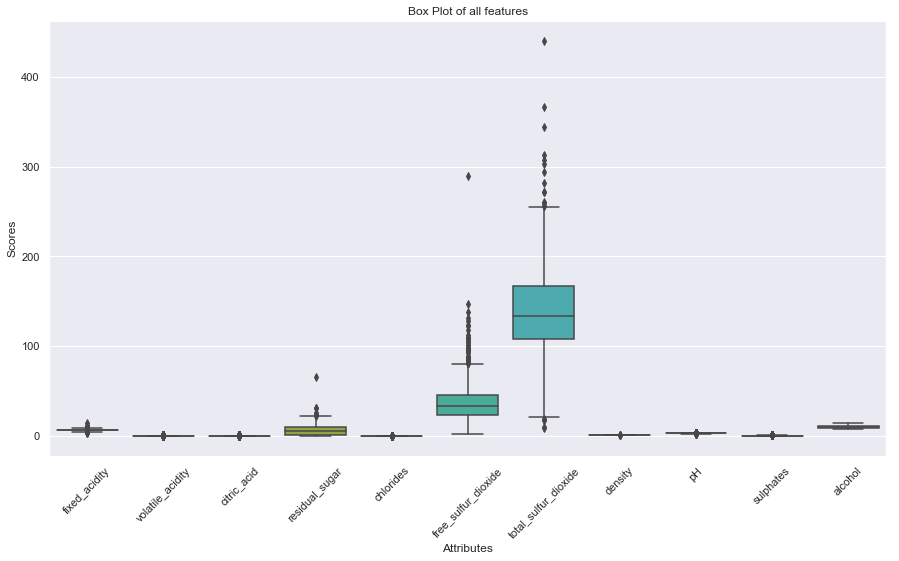
\includegraphics[totalheight=8cm]{images/boxplot-all.png}
    \caption{Boxplot showing outliers for all features.}
    \label{fig:boxplot-all}
\end{figure}

It is clear that some outliers existed. The main outliers are outlined below 

\begin{itemize}
  \item 19 total sulfur dioxide depicted in figure \ref{fig:boxplot-total_sulfor_dioxide}
  \item 7 residual sugar depicted in depicted in figure \ref{fig:boxplot-total_residual_sugar}
  \item 45 free sulfur dioxide depicted in figure \ref{fig:boxplot-free_sulfor_dioxide}
\end{itemize}

\begin{figure}[H]
\centering
        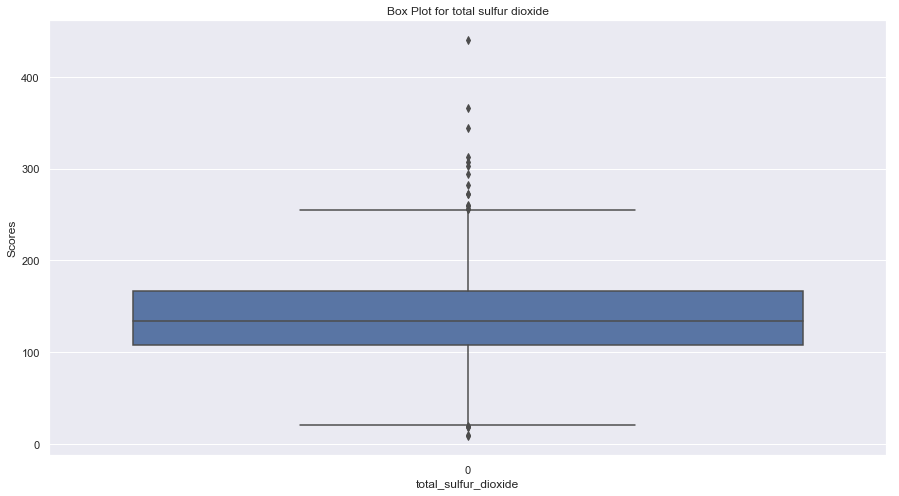
\includegraphics[totalheight=8cm]{images/boxplot-total_sulfor_dioxide.png}
    \caption{Boxplot showing outliers for all features.}
    \label{fig:boxplot-total_sulfor_dioxide}
\end{figure}

\begin{figure}[H]
\centering
        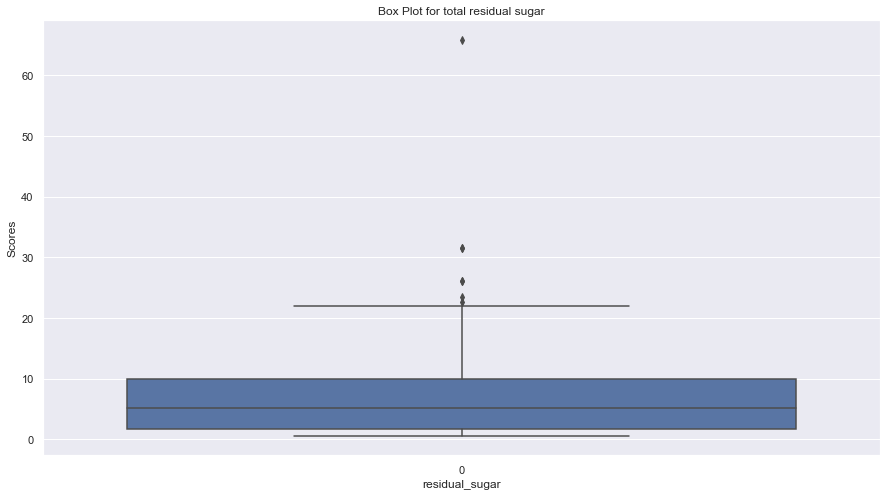
\includegraphics[totalheight=8cm]{images/boxplot-total_residual_sugar.png}
    \caption{Boxplot showing outliers for all features.}
    \label{fig:boxplot-total_residual_sugar}
\end{figure}

\begin{figure}[H]
\centering
        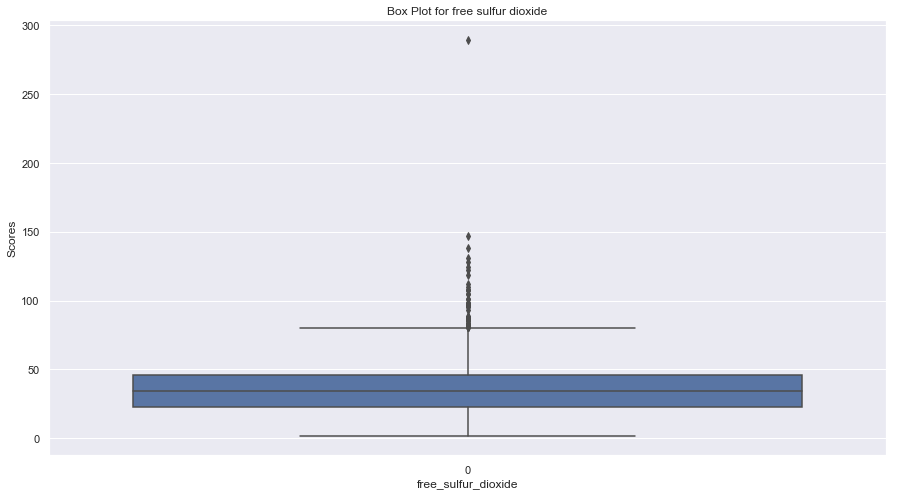
\includegraphics[totalheight=8cm]{images/boxplot-free_sulfor_dioxide.png}
    \caption{Boxplot showing outliers for all features.}
    \label{fig:boxplot-free_sulfor_dioxide}
\end{figure}

It was chosen to remove all these outliers from the dataset because there were simply not that many outliers found.

\subsection{Classification Models}

The following classification models were used to classify the quality of the wine. 

\begin{itemize}
  \item Logictic Regression
  \item Decision Tree Classification
  \item Random Forest Classification
\end{itemize}

\subsection{Hyper-Parameter Optimization}

RandomizedSearchCV was used for hyperparameter optimization. This is a very easy to use but powerful method of finding the most optimal results from a range of hyperparameters. Depending on the range of parameters this method can take a very long time to run.

For logistic regression, the following hyper-parameters were explored

\begin{itemize}
  \item C - range from 0 to 100
  \item penalty - L1 or L2
  \item fit\_intercept - True or False
  \item class\_weight - None or Balanced
  \item warm\_start - True or False
\end{itemize}

For the decision tree classifier, the following hyper-parameters were explored

\begin{itemize}
  \item criterion - Entropy or Gini
  \item max\_depth - 0 to 100
  \item class\_weight - None or Balanced
  \item min\_samples\_leaf - 1 to 5
  \item max\_features - auto, sqrt, log2 or None
\end{itemize}


For the random forest classifier, the following hyper-parameters were explored

\begin{itemize}
  \item criterion - Entropy or Gini
  \item max\_depth - 0 to 1000
  \item class\_weight - None, Balanced or balanced\_subsample
  \item min\_samples\_leaf - 1 to 5
  \item min\_samples\_split - 2 to 5
  \item max\_features - auto, sqrt, log2 or None
\end{itemize}